\documentclass[letterpaper]{article} % DO NOT CHANGE THIS
\usepackage[submission]{aaai2027} % DO NOT CHANGE THIS
\usepackage[hyphens]{url} % DO NOT CHANGE THIS
\usepackage{graphicx} % DO NOT CHANGE THIS
\urlstyle{rm} % DO NOT CHANGE THIS
\def\UrlFont{\rm} % DO NOT CHANGE THIS
\usepackage{natbib} % DO NOT CHANGE THIS AND DO NOT ADD OPTIONS
\usepackage{caption} % DO NOT CHANGE THIS AND DO NOT ADD OPTIONS
\frenchspacing % DO NOT CHANGE THIS
\setlength{\pdfpagewidth}{8.5in} % DO NOT CHANGE THIS
\setlength{\pdfpageheight}{11in} % DO NOT CHANGE THIS

\usepackage{amsmath}
\usepackage{amssymb}
\usepackage{amsthm}
\usepackage{booktabs}
\usepackage{array}
\usepackage{multirow}
\usepackage{xspace}
\usepackage{algorithm}
\usepackage{algorithmic}

\setcounter{secnumdepth}{2}
\graphicspath{{figures/}}

\newcommand{\method}{\textup{\textsc{E2E-Merge}}\xspace}
\newcommand{\norm}[1]{\left\lVert #1\right\rVert}
\newcommand{\R}{\mathbb R}

\theoremstyle{plain}
\newtheorem{theorem}{Theorem}
\newtheorem{proposition}[theorem]{Proposition}
\newtheorem{lemma}[theorem]{Lemma}
\newtheorem{corollary}[theorem]{Corollary}
\theoremstyle{definition}
\newtheorem{assumption}[theorem]{Assumption}
\newtheorem{remark}[theorem]{Remark}

\pdfinfo{
/TemplateVersion (2027.1)
}

\title{Model Consolidation under Budget:\\
From Closed-Form Merging to End-to-End Distillation}
\author{Anonymous Submission}
\affiliations{}

\begin{document}
\maketitle

\begin{abstract}
Data-assisted model consolidation is commonly approached in two computational regimes: closed-form merging, which cheaply solves parameter-space or layer-local surrogates, and multi-teacher distillation, which spends iterative computation to match expert behavior end to end.
We study when each regime is preferable rather than treating one as universally superior.
Both are organized around a task-conditioned functional objective: on inputs from task $a$, one shared model should reproduce expert $a$.
Our analysis separates the fixed \emph{surrogate gap} of closed-form regression from the data- and compute-dependent errors of end-to-end distillation.
Locally, RegMean is the exact optimizer of an expert-centered, layer-wise, first-order, isotropic surrogate; dropping cross-layer coupling incurs an exact quadratic excess loss.
Under local smoothness and Polyak--Lojasiewicz conditions, iterative refinement reduces this error with computation and admits a break-even budget, and a finite-data bound gives the complementary condition under which distillation falls below a closed-form reference.
We also show that logit distillation uses a task-head-induced semimetric, whereas representation matching supervises the full shared representation.
Existing experiments map three slices of the resulting frontier without introducing new measurements.
On ViT-B/32, RegMean++ is better with only $64$--$128$ distinct examples per task, while representation distillation overtakes it at $256$ and above and reaches $90.2\%$ against $84.2\%$ with enough updates; block-wise refinement supplies intermediate memory--accuracy points.
The distillation advantage grows with expert count and weaker backbones, whereas a preliminary Flan-T5 GLUE probe, using different functional readouts, favors closed-form RegMean.
The evidence supports a regime view: closed-form merging is preferable under severe data, compute, or memory constraints and when its surrogate is tight; end-to-end distillation pays when sufficient unlabeled data and offline computation are available and the structural gap is large.
\end{abstract}

\section{Introduction}
\label{sec:intro}

Model consolidation turns several task experts derived from a common checkpoint into one model with the original architecture and inference cost.
The literature is often described as a collection of merging algorithms, but data-assisted methods now occupy two visibly different computational regimes.
At one end, closed-form methods such as Fisher merging, RegMean, and RegMean++ collect a small set of statistics and solve a parameter- or layer-local problem once \citep{matena2022fisher,jin2023regmean,regmeanplusplus2025}.
At the other end, optimization-based mergers and multi-teacher distillation repeatedly query the experts and update a student on unlabeled inputs \citep{yang2024adamerging,prodistill2025,samerging2025}.
Both return a single consolidated model, but they trade accuracy, data, computation, and memory differently.

This paper asks a broader question than whether one particular method wins at its most accurate operating point:
\begin{quote}
\emph{When does a cheap closed-form merge suffice, and when is the additional cost of end-to-end distillation justified?}
\end{quote}
The answer cannot be reduced to accuracy divided by wall-clock time.
A practitioner may be limited by distinct unlabeled examples, student backward passes, peak activation memory, or the number and incompatibility of experts.
Moreover, the two regimes make different kinds of error.
A closed-form method can exactly solve its chosen surrogate yet remain biased for the deployed end-to-end function.
Distillation attacks that function more directly, but its finite-data and optimization errors can be large when data or iterations are scarce.

We organize both regimes around the same ideal task-conditioned functional objective.
Let $g_{\theta_a}$ be expert $a$, and let $\mathcal D_a$ be its unlabeled input distribution.
A consolidated model should reproduce expert $a$ on inputs from task $a$:
\begin{equation}
F(\theta)=\sum_{a=1}^{T}\pi_a
\mathbb E_{X\sim\mathcal D_a}
\left[\|g_\theta(X)-g_{\theta_a}(X)\|_2^2\right].
\label{eq:functional-objective}
\end{equation}
Task-conditioned multi-teacher distillation samples this objective directly.
Closed-form mergers approximate it.
In particular, RegMean is not a logit method: it performs closed-form regression on each linear layer's activations or outputs.
We show that it is the exact optimizer of an expert-centered, layer-wise, first-order surrogate after the downstream metric is replaced by a shared isotropic one.
This explains why RegMean is strong and why it may retain a fixed gap when downstream anisotropy, cross-layer coupling, merged-model activations, or nonlinear re-linearization matter.

The same framework also separates \emph{what is distilled} from \emph{how it is optimized}.
CLIP tasks use different class sets and text-prototype heads.
Logit or KL matching sees a representation only through the current head, whereas representation matching supervises a shared, head-independent space.
We characterize the exact spectral condition under which all observed heads jointly control the full representation.

The theory leads to a budgeted regime condition.
A closed-form reference has a structural functional gap $\Delta_{\mathrm{CF}}$.
End-to-end distillation with $n$ distinct examples and $K$ updates has finite-data and optimization terms.
Under a standard uniform-deviation condition, a sufficient comparison takes the form
\begin{equation}
\underbrace{2\varepsilon_n+\delta_K}_{\text{distillation: data + optimization}}
<
\underbrace{\Delta_{\mathrm{CF}}}_{\text{closed-form structural gap}},
\label{eq:regime-condition}
\end{equation}
where $\varepsilon_n$ is the empirical-to-population deviation and $\delta_K$ is empirical optimization error.
Locally, $\Delta_{\mathrm{CF}}$ is quantified by exact normal-equation, subspace, and cross-layer gap formulas; under local smoothness and a Polyak--Lojasiewicz condition, $\delta_K$ decreases geometrically in an idealized analysis.
Equation \eqref{eq:regime-condition} is not a claim that distillation always wins.
It predicts a crossover in data and computation, and it predicts that the crossover should move in favor of distillation as the closed-form surrogate becomes less accurate.

The existing experiments already expose these regimes.
On ViT-B/32, RegMean++ leads with only $64$ or $128$ distinct examples per task, but representation distillation overtakes it at $256$ and widens the gap thereafter.
Along the selected learning-rate trajectory, $4$k updates recover $83.3\%$ of the final measured gain over RegMean++, $8$k recover $98.3\%$, and the final $4$k add only $0.1$ point.
Block-wise refinement gives intermediate memory--accuracy operating points.
The gain over closed-form merging grows from $2.6$ points at two experts to $6.0$ at eight and $13.7$ at twenty on ViT-B/32, and is larger on weaker backbones for the same twenty tasks.
Conversely, the preliminary Flan-T5 GLUE probe favors closed-form RegMean ($83.0\%$) over iterative distillation ($81.9\%$), under the caveat that the two use different functional readouts.
These are precisely the kinds of crossovers a regime analysis should explain.

\paragraph{Contributions.}
\begin{itemize}
    \item We formulate closed-form merging and end-to-end distillation as two
computational regimes of task-conditioned functional consolidation.
A Bayes decomposition and a margin bound connect the objective to expert preservation.
    \item We derive an approximation--estimation--optimization view of method choice.
Exact local formulas quantify normal-equation mismatch, restricted update subspaces, and omitted cross-layer coupling; a finite-data bound and a compute-dependent descent result give sufficient break-even conditions.
    \item We distinguish target coverage from solver choice. The aggregate task heads
define a positive-semidefinite frame operator; logit supervision is equivalent to representation supervision only when it has a positive lower frame bound.
    \item Using only existing measurements, we reorganize the empirical study around
data, iteration, memory, and consolidation-difficulty frontiers.
The resulting regime map identifies where closed-form merging, block-wise refinement, and full end-to-end distillation are preferable within the studied settings.
\end{itemize}

\section{Related Work}
\label{sec:related}

\paragraph{Closed-form and parameter-space merging.}
Model soups and task arithmetic combine parameters directly \citep{wortsman2022modelsoups,ilharco2023taskarithmetic}.
TIES and DARE edit signs and sparsity \citep{yadav2023ties,yu2024dare}; TSV-M and Iso-C use task-vector subspaces \citep{gargiulo2025tsvm,marczak2025isotropic}; Fisher merging uses a diagonal sensitivity metric \citep{matena2022fisher}.
RegMean fits each linear layer by closed-form regression, and RegMean++ improves the layer inputs by propagating the partially merged network \citep{jin2023regmean,regmeanplusplus2025}.
FeatCal and Output-Space Projection further emphasize feature- or output-space calibration with efficient local solvers \citep{featcal2026,outputprojection2026}.
Closest to our local analysis, several methods cast merging as a second-order linear system: MaTS solves for merged weights using a Kronecker-factored block-diagonal Fisher approximation \citep{tam2024mats}, and uncertainty-based gradient matching relates averaging, task arithmetic, and Fisher merging through parameter-space gradient mismatch \citep{daheim2024uncertainty}.
These methods occupy low-compute operating points, but differ in the target and local geometry they retain; our exact block-diagonal and cross-layer gap formulas make precise what a layer-local or restricted second-order surrogate discards.
Curvature-based analyses have also been applied outside merging, for example to training-free structured pruning \citep{gong2026cocurve}.

\paragraph{Optimization and distillation.}
AdaMerging optimizes merge coefficients on unlabeled data \citep{yang2024adamerging}.
ProDistill performs progressive layer-wise distillation, while SAMerging formulates merging as multi-teacher logit distillation with sharpness-aware optimization \citep{prodistill2025,samerging2025}.
Classical knowledge distillation provides the general teacher--student framework \citep{hinton2015distilling}.
Our focus is not priority for using distillation.
We compare the computational regimes and characterize when the extra optimization can overcome the structural gap of a closed-form surrogate.

\paragraph{Representations and inference-time modules.}
Representation Surgery and weight-ensembling mixtures introduce feature corrections or routing at inference \citep{yang2024surgery,tang2024wemoe}.
The setting here instead returns one shared encoder with no learned router or task-specific trainable module; evaluation still chooses each task's fixed CLIP class set and text-prototype head.

\section{A Budgeted Functional View}
\label{sec:theory}

\subsection{One functional objective, two computational regimes}
\label{sec:common-objective}

Let $A$ be a task with probability $\pi_a$, draw $X\mid A=a\sim\mathcal D_a$, and set $Z=g_{\theta_A}(X)$.
Equation~\eqref{eq:functional-objective} is equivalently $F(\theta)=\mathbb E\|g_\theta(X)-Z\|_2^2$.
Its unconstrained Bayes target is $\mu(x)=\mathbb E[Z\mid X=x]$, and
\begin{equation}
F(h)=\mathbb E\|h(X)-\mu(X)\|_2^2
+\mathbb E\|Z-\mu(X)\|_2^2.
\label{eq:bayes-main}
\end{equation}
The second term is irreducible conflict among experts on overlapping inputs.
The first is what a shared model can reduce.
A margin argument further gives, for every $\gamma_0>0$,
\begin{equation}
|\mathrm{Acc}_a(\theta)-\mathrm{Acc}_a(\theta_a)|
\le
\Pr[\gamma_a(X)\le\gamma_0]
+\frac{4F_a(\theta)}{\gamma_0^2},
\label{eq:accuracy-main}
\end{equation}
where $F_a$ is task $a$'s representation loss and $\gamma_a$ is the expert top-two margin.
Thus the functional discrepancy is aligned with preserving the experts, though it is not identical to ground-truth accuracy.

Closed-form and iterative methods address Eq.~\eqref{eq:functional-objective} differently.
A closed-form method selects a surrogate $\widetilde F$ that can be solved analytically or with a small linear system.
Its optimization error on $\widetilde F$ is negligible, but its output can retain a structural gap on $F$.
Distillation uses samples of $F$ itself, but must estimate and optimize it.
This yields the schematic comparison
\begin{equation}
\begin{aligned}
\mathcal E_{\mathrm{CF}}(n)
&\approx \Delta_{\mathrm{sur}}+\Delta_{\mathrm{est}}^{\mathrm{CF}}(n),\\
\mathcal E_{\mathrm{Dist}}(n,K)
&\approx \Delta_{\mathrm{est}}^{\mathrm{Dist}}(n)
+\Delta_{\mathrm{opt}}(K).
\end{aligned}
\label{eq:schematic-errors}
\end{equation}
Equation~\eqref{eq:schematic-errors} is an organizing decomposition, not an exact equality for arbitrary neural networks.
The next results make its structural and optimization parts precise under local assumptions.

\subsection{The fixed structural gap of closed-form regression}
\label{sec:closed-form-gap}

Around a reference merge $\bar\theta$, linearize the residual and add damping:
\begin{equation}
Q(\Delta)=C-b^\top\Delta+\tfrac12\Delta^\top H\Delta,
\qquad H\succ0.
\label{eq:local-quadratic}
\end{equation}
The full local optimum is $\Delta^\star=H^{-1}b$.
For any surrogate update $\widetilde\Delta$,
\begin{equation}
Q(\widetilde\Delta)-Q(\Delta^\star)
=\tfrac12\|H\widetilde\Delta-b\|_{H^{-1}}^2.
\label{eq:gap-main}
\end{equation}
If the surrogate solves $\widetilde H\widetilde\Delta=\widetilde b$, the residual becomes $(H-\widetilde H)\widetilde\Delta+(\widetilde b-b)$, separating geometry from trajectory/target mismatch.
If $H=D+E$ and a layer-wise method keeps only the block diagonal $D$, its exact local excess is
\begin{equation}
Q(\Delta_D)-Q(\Delta^\star)
=\tfrac12\|E\Delta_D\|_{H^{-1}}^2,
\qquad \Delta_D=D^{-1}b.
\label{eq:cross-layer-gap-main}
\end{equation}
Likewise, restricting updates to $\Delta=Uc$ for a coefficient vector $c$ loses the $H$-energy of the unrestricted solution outside $\operatorname{col}(U)$.

\begin{proposition}[Local structural gap]
\label{prop:local-gap-main}
Let $Q$ be given by Eq.~\eqref{eq:local-quadratic}.
If a surrogate returns $\widetilde\Delta$ by solving $\widetilde H\widetilde\Delta=\widetilde b$, then its excess local functional loss is exactly \[ \frac12\left\|(H-\widetilde H)\widetilde\Delta+(\widetilde b-b)\right\|_{H^{-1}}^2.
\] For a block-diagonal approximation $D$ this reduces to $\tfrac12\|E\Delta_D\|_{H^{-1}}^2$, and for a restricted subspace it equals the $H$-energy of the full update outside that subspace.
\end{proposition}

The proposition separates three quantities that are otherwise conflated in a method-level comparison: the target or trajectory used to form $b$, the geometry retained in $H$, and the space in which an update is allowed to move.
It is a local objective statement, not a claim that a nonlinear optimizer reaches the global optimum.

RegMean is a concrete specialization.
It solves, independently for each layer,
\begin{equation}
\begin{aligned}
W_{\mathrm{RM}}
&=\arg\min_W \sum_a\|(W-W_a)X_a\|_F^2,\\
&=\left(\sum_aW_aX_aX_a^\top\right)
  \left(\sum_aX_aX_a^\top\right)^{-1}.
\end{aligned}
\label{eq:regmean-main}
\end{equation}
It is the exact minimizer of an expert-centered, one-layer, first-order surrogate when the downstream metric is replaced by a shared scaled identity.
It is therefore a closed-form \emph{activation-regression} method, not logit optimization.
RegMean++ reduces the activation-trajectory mismatch but remains layer local.
End-to-end refinement can exploit the downstream metric, off-diagonal blocks, current merged activations, and repeated nonlinear re-linearization that Eq.~\eqref{eq:regmean-main} omits.

\subsection{When iterative distillation pays}
\label{sec:compute-error-main}

Let $F^\star=\inf_\theta F(\theta)$ and define a closed-form reference gap $\Delta_{\mathrm{CF}}=F(\theta_{\mathrm{CF}})-F^\star$.
For idealized full-gradient updates on an $L$-smooth region,
\begin{equation}
F(\theta_K)
\le F(\theta_0)-\frac{\eta}{2}
\sum_{k=0}^{K-1}\|\nabla F(\theta_k)\|_2^2,
\qquad 0<\eta\le 1/L.
\label{eq:compute-descent-main}
\end{equation}
If the same region satisfies a Polyak--Lojasiewicz condition \citep{karimi2016pl} with constant $\mu>0$,
\begin{equation}
F(\theta_K)-F^\star
\le(1-\mu\eta)^K\bigl(F(\theta_0)-F^\star\bigr).
\label{eq:compute-rate-main}
\end{equation}
A sufficient local break-even budget is therefore
\begin{equation}
K_{\mathrm{be}}=
\left\lceil
\frac{\log(\Delta_{\mathrm{CF}}/\Delta_0)}
     {\log(1-\mu\eta)}
\right\rceil,
\label{eq:break-even-main}
\end{equation}
when $0<\Delta_{\mathrm{CF}}<\Delta_0$, where $\Delta_0=F(\theta_0)-F^\star$ is the initial functional gap.
These statements idealize full-gradient descent; they are not convergence guarantees for AdamW.

Data adds a second axis.
Let $\widehat F_n$ be the empirical functional objective over $n$ distinct examples and suppose $\sup_{\theta\in\mathcal R}|F(\theta)-\widehat F_n(\theta)|\le\varepsilon_n$ on the relevant region.
If an iterate has empirical optimization error $\delta_K$, then
\begin{equation}
F(\theta_K)-F^\star\le 2\varepsilon_n+\delta_K.
\label{eq:finite-data-bound-main}
\end{equation}
Consequently, Eq.~\eqref{eq:regime-condition} is a sufficient condition for distillation to beat the chosen closed-form reference.
It predicts that small $n$ favors the stable closed-form estimator, increasing $K$ reduces optimization error, and a larger structural gap moves the crossover toward distillation.

\subsection{Representation versus logit distillation}
\label{sec:head-coverage}

For task $a$, let $T_a$ collect its CLIP text prototypes.
A representation error $v$ is seen by squared-logit matching as $\|T_a^\top v\|_2^2$.
For nonnegative weights $\omega_a$, define $S=\sum_a\omega_aT_aT_a^\top$.
Then
\begin{equation}
\lambda_{\min}(S)\|v\|_2^2
\le\sum_a\omega_a\|T_a^\top v\|_2^2
\le\lambda_{\max}(S)\|v\|_2^2.
\label{eq:frame-main}
\end{equation}
The aggregate logit seminorm controls the full representation exactly when $S\succ0$; if $S$ is singular, a nonzero direction is invisible to every included head.
Local KL matching induces the related metric $T_a(\operatorname{Diag}p_a-p_ap_a^\top)T_a^\top$, where $p_a$ is the teacher's softmax distribution.
Representation matching instead uses the identity metric in the shared representation space.
This target distinction is orthogonal to the closed-form-versus-iterative distinction.

\subsection{Predicted operating regimes}
\label{sec:predictions}

The analysis predicts four qualitative regimes.
First, extreme sample scarcity favors closed form because distillation's estimation error is large.
Second, with sufficient data, iterative refinement should cross the fixed surrogate and then show diminishing returns.
Third, as the structural gap grows, for example when more experts must be consolidated or a weaker backbone has less slack, the crossover should favor distillation.
Fourth, block-wise refinement should interpolate between closed-form memory and full end-to-end accuracy.
The experiments report one-dimensional slices of this multi-resource frontier; they do not estimate a universal hardware-independent scalar ``efficiency score.'' Table~\ref{tab:regime-comparison} summarizes the compared regimes and their characteristic residual errors.

\begin{table*}[tb]
\centering
\small
\setlength{\tabcolsep}{4pt}
\begin{tabular}{p{0.16\textwidth}p{0.20\textwidth}p{0.18\textwidth}p{0.17\textwidth}p{0.20\textwidth}}
\toprule
Regime & Matched quantity & Update scope & Solver and dominant cost & Characteristic residual error \\
\midrule
RegMean family & Per-layer activations or outputs & One linear layer at a time & Statistics pass plus closed-form solves & Fixed layer-local, isotropic, and cross-layer approximation gap \\
Logit distillation & Task-specific probabilities/logits & All student weights & Teacher forward plus student forward/backward per step & Head-induced semimetric may leave representation directions unconstrained \\
Representation distillation & Shared final representation & All student weights & Teacher forward plus student forward/backward per step & Finite-data and iterative optimization error on the end-to-end objective \\
Block-wise refinement & Intermediate/final representations & Consecutive block groups & Iterative, with cached frozen prefixes & Intermediate cross-block approximation and memory cost \\
\bottomrule
\end{tabular}
\caption{The compared regimes differ in both the target and the computational mechanism.
RegMean is activation regression rather than logit optimization.
The empirical study therefore separates target choice inside the iterative family from the broader closed-form-to-end-to-end comparison.}
\label{tab:regime-comparison}
\end{table*}

\section{Representative Operating Points}
\label{sec:method}

\paragraph{Closed-form endpoint.}
RegMean++ is the main low-compute reference.
It collects activation statistics while propagating a partially merged network and solves each linear layer in closed form.
The reported implementation takes on the order of a minute after its statistics pass.

\paragraph{End-to-end endpoint.}
Our high-accuracy operating point, \method, initializes the student by task arithmetic, freezes all experts, samples a task and minibatch, and minimizes
\begin{equation}
\mathcal L(\theta;x,a)=
\left\|g_\theta(x)-\operatorname{sg}\!\bigl(g_{\theta_a}(x)\bigr)\right\|_2^2,
\label{eq:method-loss}
\end{equation}
where $g$ is the normalized projected CLIP representation and $\operatorname{sg}$ is stop-gradient.
We use AdamW and update all encoder weights (Algorithm~\ref{alg:e2e}).
The procedure is label-free but data-assisted and repeatedly queries the teachers.

\begin{algorithm}[tb]
\caption{End-to-end representation distillation (\method)}
\label{alg:e2e}
\begin{algorithmic}[1]
\REQUIRE Pre-trained $\theta_0$, experts $\{\theta_a\}_{a=1}^T$, unlabeled loaders,
steps $K$, scale $\alpha$
\STATE $\theta\leftarrow\theta_0+\alpha\sum_a(\theta_a-\theta_0)$
\STATE Freeze all experts
\FOR{$k=1$ to $K$}
    \STATE Sample task $a$ and batch $x\sim\mathcal D_a$
    \STATE $z\leftarrow\operatorname{sg}(g_{\theta_a}(x))$
    \STATE Update $\theta$ with AdamW on $\|g_\theta(x)-z\|_2^2$
\ENDFOR
\RETURN $\theta$
\end{algorithmic}
\end{algorithm}

\paragraph{Intermediate memory points.}
The block-wise variant trains consecutive block groups from the input side while freezing and caching the prefix.
Group size controls joint nonlinear scope and activation memory.
It is not closed form, but it creates intermediate operating points between RegMean++ and full end-to-end refinement.

\section{Experiments: Mapping the Accuracy--Efficiency Frontier}
\label{sec:experiments}

\subsection{Setup}
All CLIP experiments use FusionBench with the same public experts, data loading, and test protocol \citep{tang2024fusionbench}.
We study the standard eight tasks on ViT-B/32, ViT-B/16, and ViT-L/14, and the TALL-20 extension \citep{ilharco2023taskarithmetic,wang2024tall}.
Data-driven methods use unlabeled training inputs; test labels are used only for evaluation.
\method uses task-arithmetic scale $0.3$, AdamW, learning rate $5\times10^{-6}$, gradient clipping $1.0$, and batch size $32$ ($16$ for TALL-20).
Measured full-run costs appear in Table~\ref{tab:measured-cost-main}; further protocols, per-task results, and seeds are provided in the technical supplement.

\begin{table}[tb]
\centering
\small
\setlength{\tabcolsep}{3.5pt}
\begin{tabular*}{\columnwidth}{@{\extracolsep{\fill}}lrrr}
\toprule
Setting & Steps & Minutes & Peak GB \\
\midrule
B/32, 8 experts & 12k & $\sim35$ & $\sim8$ \\
L/14, 8 experts & 8k & $\sim13$ & $\sim31$ \\
L/14, 20 experts & 16k & $\sim34$ & $\sim24$ \\
\bottomrule
\end{tabular*}
\caption{Measured full-run cost of representation distillation on one RTX 6000 Ada.
Closed-form RegMean++ remains roughly minute-scale after its statistics pass; the table does not interpolate unmeasured intermediate wall-clock values.}
\label{tab:measured-cost-main}
\end{table}

\subsection{Accuracy endpoints}

\begin{table*}[tb]
\centering
\small
\setlength{\tabcolsep}{5pt}
\begin{tabular}{l l c c c}
\toprule
Setting & Best evaluated closed-form reference & Reference acc. & End-to-end acc. & Difference \\
\midrule
ViT-B/32, 8 experts & RegMean++ & 84.2 & $89.8\pm0.4$ & $+5.6$ \\
ViT-B/16, 8 experts & RegMean++ & 87.3 & 92.0 (single run) & $+4.7$ \\
ViT-L/14, 8 experts & RegMean++ & 90.9 & $94.2\pm0.1$ & $+3.3$ \\
ViT-L/14, 20 experts & Iso-C & 83.4 & $92.9\pm0.2$ & $+9.5$ \\
\bottomrule
\end{tabular}
\caption{High-accuracy endpoints under the common harness. The ViT-B/32 and ViT-L/14
representative longer runs reach $90.2\%$ and $94.3\%$, respectively; the table uses the available multi-seed means as the primary values.
``Closed-form reference'' denotes the strongest evaluated non-iterative method in each row.}
\label{tab:accuracy-endpoints}
\end{table*}

The endpoint results (Table~\ref{tab:accuracy-endpoints}) establish that iterative representation distillation can substantially raise the accuracy ceiling, but they do not by themselves establish efficiency.
We therefore examine separate data, update, and memory slices (Figure~\ref{fig:budget-frontiers}).

\subsection{Data, iteration, and memory crossovers}

\begin{figure*}[tb]
\centering
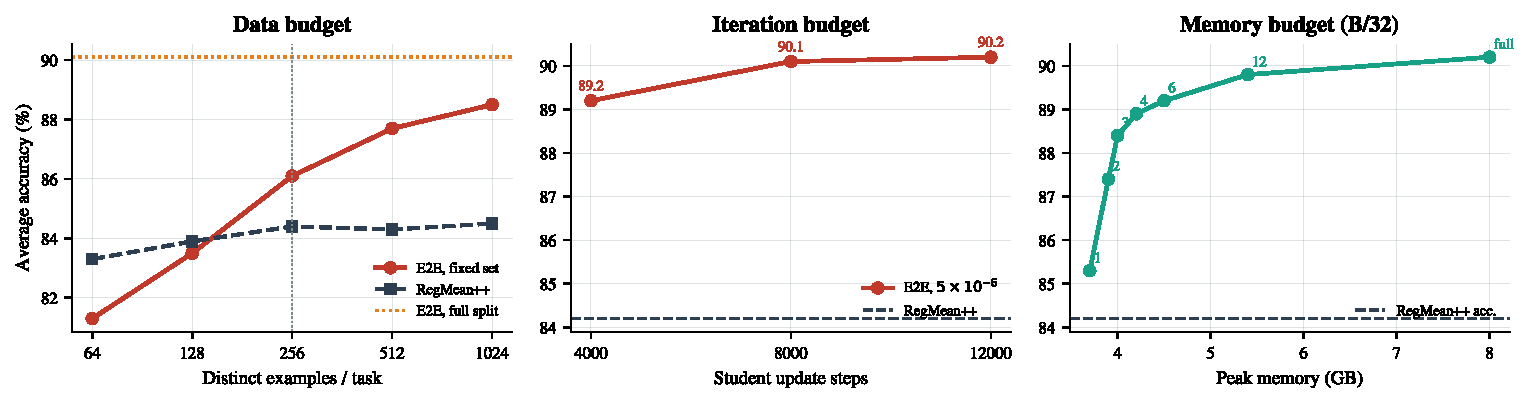
\includegraphics[width=0.98\textwidth]{fig_budget_frontiers.pdf}
\caption{Three measured slices of the accuracy--efficiency frontier, all from existing
ViT-B/32 results.
Left: with a fixed set, RegMean++ leads at $64$--$128$ distinct examples per task, while end-to-end refinement crosses it at $256$; full-split reshuffling reaches $90.1\%$.
Middle: at the selected learning rate, $4$k, $8$k, and $12$k student updates reach $89.2\%$, $90.1\%$, and $90.2\%$ versus RegMean++ at $84.2\%$.
Right: block-wise and canonical full refinement trade peak memory for accuracy; labels denote jointly optimized blocks, and ``full'' is the canonical approximately $8$ GB endpoint.
These are one-dimensional slices, not a jointly compute-matched Pareto surface.}
\label{fig:budget-frontiers}
\end{figure*}

\paragraph{Data frontier.}
At $N=64$ and $128$ distinct examples per task, RegMean++ obtains $83.3\%$ and $83.9\%$, above the fixed-set E2E values $81.3\%$ and $83.5\%$.
At $N=256$, the ordering reverses: $86.1\%$ versus $84.4\%$, and the E2E lead grows to $3.4$ and $4.0$ points at $512$ and $1024$.
This is the cleanest observed regime crossover: an analytic regression estimate is more sample efficient under extreme scarcity, whereas the more expressive objective pays once enough distinct inputs are available.
The methods use the same unique examples at each $N$, but not the same sample exposure or compute.

\paragraph{Iteration frontier.}
For the selected $5\times10^{-6}$ learning rate, the existing $4$k, $8$k, and $12$k measurements yield the sequence in Table~\ref{tab:step-increments}.
\begin{table}[tb]
\centering
\small
\setlength{\tabcolsep}{4pt}
\begin{tabular*}{\columnwidth}{@{\extracolsep{\fill}}lrrr}
\toprule
Point & Updates & Acc. & Gain \\
\midrule
RegMean++ & closed form & 84.2 & 0.0 \\
\method & 4k & 89.2 & $+5.0$ \\
\method & 8k & 90.1 & $+5.9$ \\
\method & 12k & 90.2 & $+6.0$ \\
\bottomrule
\end{tabular*}
\caption{Observed ViT-B/32 accuracy--step slice. Step count is a within-\method compute
proxy, not a wall-clock match to RegMean++; the full 12k run takes about 35 minutes.}
\label{tab:step-increments}
\end{table}
The $4$k point already recovers $5.0/6.0=83.3\%$ of the final measured improvement, and $8$k recovers $5.9/6.0=98.3\%$.
The curve therefore displays the predicted crossing and diminishing returns.
We do not infer unmeasured intermediate wall-clock values or fit the theoretical convergence constants.

\paragraph{Memory frontier.}
On ViT-B/32, block-wise refinement moves from $85.3\%$ at $3.7$ GB to $89.8\%$ at $5.4$ GB, with the canonical full run at $90.2\%$ and about $8$ GB.
On ViT-L/14, a single-block schedule reaches $92.0\%$ at about $13$ GB, four-block groups reach $93.0\%$ at about $15$ GB, and the full block-wise run reaches $94.2\%$ at about $31$ GB.
These points show that memory-constrained users need not choose only between closed form and full-network backpropagation.

\subsection{The crossover moves with consolidation difficulty}
\label{sec:difficulty-frontier}

On ViT-B/32, the \method--RegMean++ gap increases from $2.6$ points at two experts to $3.3$ at four, $4.4$ at six, $6.0$ at eight, and $13.7$ at twenty (Figure~\ref{fig:scaling-main}).
For the same twenty TALL tasks, the margin over the best evaluated baseline is $9.5$ on ViT-L/14, $12.0$ on ViT-B/16, and $13.7$ on ViT-B/32.
These are operational stress axes rather than a proof of a universal scalar interference law, but they agree with the structural-gap account: when a local or restricted compromise is farther from the shared end-to-end function, additional distillation compute buys more.

\begin{figure}[tb]
\centering
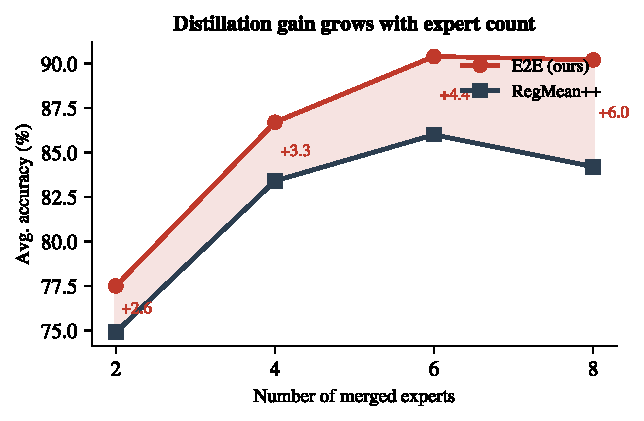
\includegraphics[width=0.94\columnwidth]{fig_scaling.pdf}
\caption{Average ViT-B/32 accuracy as the number of merged experts increases. The
\method--RegMean++ margin grows from $2.6$ to $6.0$ points across the reported two- to eight-expert subsets; the twenty-expert margin is $13.7$ points.}
\label{fig:scaling-main}
\end{figure}

The preliminary Flan-T5 GLUE study supplies the opposite case.
Closed-form RegMean reaches $83.0\%$, while iterative E2E matching reaches $81.9\%$; both beat task arithmetic ($79.0\%$) and TIES ($80.2\%$).
Because RegMean matches layer activations whereas the E2E variant matches the first-step output distribution, this is not a like-for-like solver comparison.
It nevertheless demonstrates that the iterative endpoint is not universally best and motivates the regime view rather than an unconditional ranking.

\subsection{Target choice and the structural mechanism}

\begin{table}[tb]
\centering
\small
\setlength{\tabcolsep}{4pt}
\begin{tabular}{llrr}
\toprule
Backbone & Initialization & Logit KL & Representation \\
\midrule
ViT-B/32 & pre-trained & 87.9 & 89.5 \\
ViT-B/32 & task arithmetic & 88.0 & 90.2 \\
ViT-L/14 & pre-trained & 92.3 & 94.1 \\
ViT-L/14 & task arithmetic & 92.2 & 94.3 \\
\bottomrule
\end{tabular}
\caption{Target-by-initialization control at matched settings within the iterative family.
Representation matching adds $1.6$--$2.2$ points, while the merge initialization adds at most $0.7$ point.
An in-harness sharpness-aware logit control (KL$+$SAM, best over a $\rho$ sweep) reaches $89.1$ on ViT-B/32 and $92.9$ on ViT-L/14, still below representation matching, so the target gap is not an artifact of omitting sharpness-aware optimization.}
\label{tab:target-init-main}
\end{table}

The target control (Table~\ref{tab:target-init-main}) supports the head-coverage analysis: representation supervision is the main within-family contributor, not initialization.
The comparison with RegMean++ is broader and simultaneously changes the target scope, update space, trajectory, solver, and compute; it should be read as the overall closed-form-to-end-to-end regime gap, not the isolated effect of gradients.
Indeed, gradient computation alone is not sufficient: the gradient-based coefficient merger AdaMerging reaches only $82.6$ under the same harness, below closed-form RegMean++.

\begin{figure*}[tb]
\centering
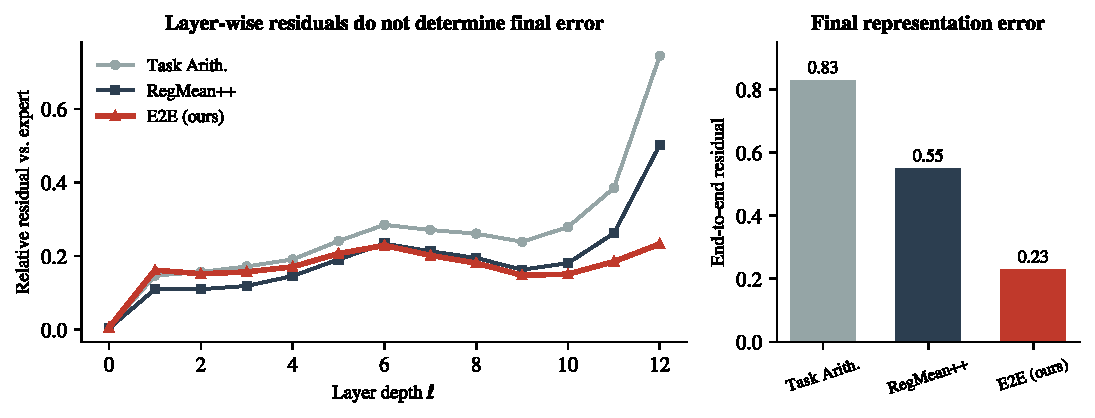
\includegraphics[width=0.72\textwidth]{fig_compound.pdf}
\caption{Layer-wise and final residuals on ViT-B/32. RegMean++ and \method have similar
summed layer-wise residuals ($2.46$ versus $2.11$), but final representation residuals of $0.55$ and $0.23$.
The post-hoc diagnostic uses test inputs only after all model and hyperparameter choices were fixed.}
\label{fig:compound}
\end{figure*}

The residual measurement (Figure~\ref{fig:compound}) explains why the higher-compute endpoint can improve: the local regression objective is already small, yet it does not determine the final functional error.
Across task arithmetic, RegMean++, and \method, final residuals $0.83$, $0.55$, and $0.23$ follow the accuracy ordering $67.6$, $84.2$, and $90.2$, whereas the summed layer-wise residual does not.

\subsection{Held-out transfer and statistical stability}
\label{sec:heldout-main}
A budgeted comparison must also check that iterative fitting does not merely trade seen-task accuracy for unseen-task degradation.
Under the two held-out splits used by AdaMerging (Table~\ref{tab:heldout-main}), the end-to-end model obtains seen/unseen averages of $87.0/66.4$ and $88.4/53.9$.
On the seen tasks it leads the best baseline (RegMean++, at $81.7$ and $84.2$) by more than five points, while on the unseen tasks it matches the best baseline (Iso-C, at $65.8$ and $53.3$) to within seed variation.
The supported conclusion is therefore the absence of a measurable seen--unseen penalty rather than a claim of improved zero-shot transfer.

\begin{table}[tb]
\centering
\small
\setlength{\tabcolsep}{3pt}
\begin{tabular*}{\columnwidth}{@{\extracolsep{\fill}}lrrrr}
\toprule
& \multicolumn{2}{c}{Split 1} & \multicolumn{2}{c}{Split 2} \\
Method & Seen & Unseen & Seen & Unseen \\
\midrule
Task Arithmetic & 69.9 & 58.1 & 73.2 & 48.8 \\
Iso-C & 77.0 & 65.8 & 80.2 & 53.3 \\
TSV-M & 81.1 & 65.7 & 83.6 & 51.2 \\
RegMean++ & 81.7 & 63.1 & 84.2 & 52.4 \\
\method & \textbf{87.0} & \textbf{66.4} & \textbf{88.4} & \textbf{53.9} \\
\bottomrule
\end{tabular*}
\caption{Held-out protocol on ViT-B/32: merge six seen experts and evaluate six seen and two unseen tasks. The unseen differences are within seed variation.}
\label{tab:heldout-main}
\end{table}

The available repeated runs give $89.8\pm0.4$ on ViT-B/32, $94.2\pm0.1$ on ViT-L/14, and $92.9\pm0.2$ on TALL-20.
The representative longer ViT-B/32 and ViT-L/14 runs reach $90.2$ and $94.3$; we use the multi-seed means for headline comparisons and retain the longer runs only as measured frontier endpoints.

\paragraph{Deployment contract.}
All operating points return one shared encoder with no learned router or task-specific trainable module, so the additional cost is paid only once before deployment.
CLIP evaluation still selects the fixed class set and text-prototype head associated with each task; ``one model'' therefore refers to the shared encoder rather than a task-agnostic label space.
Inference architecture and encoder cost are unchanged across the compared operating points.

\subsection{Practical choice within the studied settings}

\begin{table}[tb]
\centering
\small
\setlength{\tabcolsep}{4pt}
\begin{tabular}{p{0.63\columnwidth}p{0.29\columnwidth}}
\toprule
Observed evidence & Suggested point \\
\midrule
RegMean++ leads at $N=64,128$ & Closed form \\
E2E crosses at $N=256$ and improves with $N$ & Full E2E \\
Peak-memory budget between the endpoints & Block-wise \\
TALL-20 margins grow to $9.5$--$13.7$ points & Favor E2E \\
GLUE: RegMean $83.0$ vs. E2E $81.9$ (different targets) & Retain closed form \\
\bottomrule
\end{tabular}
\caption{Empirical regime map within the studied settings. It is a decision aid, not a
universal theorem or an exhaustive field-wide comparison.}
\label{tab:regime-map}
\end{table}

\paragraph{A conservative decision procedure.}
Table~\ref{tab:regime-map} collects the observed evidence and the suggested operating point.
Within the measured CLIP setting, start from a closed-form solution when the calibration set is tiny or only statistics-pass compute is available.
At $256$ distinct examples per task, end-to-end refinement becomes more accurate in the ViT-B/32 sweep.
A $4$k-step run captures most of the final measured gain and $8$k is near the observed plateau.
Under activation-memory constraints, block-wise refinement supplies intermediate points.
The larger gains for twenty experts and weaker backbones suggest prioritizing iterative budget where the local compromise is most stressed.
These thresholds are benchmark-specific and should be re-estimated for a new architecture.

\subsection{Reporting efficiency without a fragile scalar score}
\label{sec:efficiency-metrics}
A ratio such as accuracy divided by minutes is not invariant to the accuracy origin, hardware, or resource being constrained.
We instead recommend reporting a resource vector $r=(n,K,M,t)$ of distinct examples, student updates, peak memory, and wall-clock, and comparing methods by Pareto dominance over accuracy and every reported resource.
Under a single scalar budget $B$ one may summarize by the budgeted envelope $A^\star(B)=\max_{m:\,C_m\le B}A_m$ for a concrete resource $C_m$, or by the cost $C_m(\epsilon)=\min\{C:A_{\mathrm{expert}}-A_m(C)\le\epsilon\}$ to reach an expert-relative gap $\epsilon$.
The present data support separate slices in $n$, $K$, and $M$ plus three measured endpoint times, not a fully joint Pareto surface or unmeasured wall-clock interpolation, so the regime map is evidence rather than a universal hardware-independent ranking.

\section{Conclusion}
\label{sec:conclusion}

Closed-form merging and end-to-end distillation are best viewed as different budget regimes of functional model consolidation.
Closed-form regression spends little compute and exactly solves a local surrogate, which is advantageous under severe sample or compute constraints and when that surrogate is tight.
Distillation spends teacher queries and student backward passes to reduce the end-to-end functional discrepancy; it becomes worthwhile once its finite-data and optimization errors fall below the closed-form structural gap.
Existing measurements reveal this crossover across data, iteration, memory, expert count, backbone strength, and a preliminary language-model probe: the result is not a universal winner, but a practical accuracy--efficiency frontier with closed-form, block-wise, and full end-to-end operating points.

\clearpage
\bibliography{references}

\end{document}
